%! TEX root = **/000-main.tex
% vim: spell spelllang=en:


\subsection{Normalized arccosine kernels}

As explained in \cref{sub:kernel_normalization_acos}, the normalization of the
arccosine kernel makes the kernels insensitive to the scaling of the input data
proposed by \cite{pandeyGoDeepWide2014} as a way of introducing the $\sigma$
hyperparameter. This means that for the normalized arccosine kernel, there is
no $\sigma$ hyperparameter to tune. Additionally, for $n=0$, the kernel is
already normalized.

We can perform the paired t-test between the results obtained with each of the
normalized arccosine kernels and the radial basis kernel. Taking the best
performant hyperparamters (the ones that minimize the nRMSE) for each kernel and
dataset combination.

\subsubsection{Normalized Arccosine kernel for $n=0$}

\Cref{tab:paired_ttest_acos0_rbf} shows the results for the paired t-test of
the normalized arccosine kernel for $n=0$ against the radial basis kernel. Looking
at the $p$\textendash{}values, we can see that for most datasets, the null hypothesis
cannot be rejected, which means that we cannot reject the hypothesis that both
kernels perform the same. In bold, we highlight the $p$\textendash{}values that
reject the null hypothesis with a significance level of $\alpha = 0.001$. In all
these cases except for the \texttt{Pumadyn32nm} dataset, the RBF kernel performs
better than the normalized arccosine kernel for $n=0$.

\begin{table}[H]
    \caption{Results for the paired t-test of acos $n=0$ against RBF for regression datasets}
    \label{tab:paired_ttest_acos0_rbf}
    %! TEX root = **/000-main.tex
% vim: spell spelllang=en:
%
\begin{tabular}{lrrr}
	\toprule
	\textbf{DataSet}                          & \textbf{$p$\textendash{}value} & \textbf{$t$\textendash{}stat} & \textbf{$\Delta$nRMSE (RBF - Acos0)} \\\midrule
	Abalone                                   & 0.39                           & 0.95                          & 0.0014                               \\
	Ailerons                                  & \textbf{1.0e-5}                & 18.0                          & -0.12                                \\
	AutoMpg                                   & 0.32                           & 1.1                           & -0.034                               \\
	Bank32fh                                  & 0.25                           & -1.3                          & 0.0005                               \\
	Bank32fm                                  & \textbf{0.00016}               & 10.0                          & -0.019                               \\
	\addlinespace
	Bank32nh                                  & 0.054                          & 2.5                           & -0.013                               \\
	Bank32nm                                  & \textbf{1.2e-5}                & 17.0                          & -0.055                               \\
	Bank8fh                                   & \textbf{0.00011}               & 11.0                          & -0.03                                \\
	Bank8fm                                   & \textbf{2.7e-5}                & 15.0                          & -0.065                               \\
	Bank8nh                                   & \textbf{0.00042}               & 8.3                           & -0.04                                \\
	\addlinespace
	Bank8nm                                   & \textbf{4.0e-6}                & 21.0                          & -0.23                                \\
	% BikeSharingDay          & \textbf{1.8e-9}                & 100.0                         & -1.0                                 \\
	% BikeSharingHour         & \textbf{2.4e-9}                & 96.0                          & -1.9                                 \\
	CPU                                       & 0.034                          & 2.9                           & -0.54                                \\
	Cancer                                    & 0.47                           & 0.78                          & 0.01                                 \\
	CommunitiesAndCrime                       & 0.0015                         & 6.3                           & -0.6                                 \\
	CompActs                                  & 0.088                          & 2.1                           & -0.051                               \\
	\addlinespace
	EatingHabits                              & 0.0015                         & 6.3                           & -0.68                                \\
	Elevators                                 & 0.17                           & 1.6                           & 0.0023                               \\
	% EnergyEfficiencyCooling & \textbf{3.1e-5}                & 14.0                          & -0.91                                \\
	% EnergyEfficiencyHeating & \textbf{7.8e-8}                & 48.0                          & -0.94                                \\
	% LiverDisorders       & 0.29                           & 1.2                           & -1.1                                 \\
	Pumadyn32fh                               & 0.74                           & 0.35                          & -0.00074                             \\
	Pumadyn32fm                               & 0.1                            & -2.0                          & 0.0064                               \\
	Pumadyn32nh                               & 0.0037                         & -5.1                          & 0.021                                \\
	\addlinespace
	\rowcolor[gray]{0.85}\textbf{Pumadyn32nm} & \textbf{0.00058}               & -7.7                          & \textbf{0.038}                       \\
	Pumadyn8fh                                & 0.031                          & 3.0                           & -0.0079                              \\
	Pumadyn8fm                                & \textbf{4.5e-5}                & 13.0                          & -0.037                               \\
	Pumadyn8nh                                & \textbf{0.00022}               & 9.5                           & -0.068                               \\
	Pumadyn8nm                                & \textbf{4.2e-8}                & 54.0                          & -0.16                                \\
	\addlinespace
	Stock                                     & 0.41                           & -0.9                          & 0.0048                               \\
	Triazines                                 & 0.96                           & 0.058                         & -0.0064                              \\\bottomrule
\end{tabular}

\end{table}

\subsubsection{Normalized Arccosine kernel for $n=1$}

\cref{tab:paired_ttest_acos1_rbf} shows the results for the paired t-test of
the normalized arccosine kernel for $n=1$ against the radial basis kernel in the
same format as \cref{tab:paired_ttest_acos0_rbf}. In this case, there are no
datasets where the arccosine kernel outperforms the RBF kernel in a statistically
significant way. Comparing the $p$\textendash{}values with the ones obtained
in \cref{tab:paired_ttest_acos0_rbf}, we can see that they are in the same order
of magnitude for most datasets. In fact, the datasets in which the $p$\textendash{}values
reject the null hypothesis are the same, except for the \texttt{Pumadyn32nm}, which
for $n=1$ the null hypothesis cannot be rejected.

\begin{table}[H]
    \caption{Results for the paired t-test of acos $n=1$ against RBF for regression datasets}
    \label{tab:paired_ttest_acos1_rbf}
    %! TEX root = **/000-main.tex
% vim: spell spelllang=en:
%
\begin{tabular}{lrrr}
	\toprule
	\textbf{DataSet}    & \textbf{$p$\textendash{}value} & \textbf{$t$\textendash{}stat} & \textbf{$\Delta$nRMSE (RBF - Acos1)} \\\midrule
	Abalone             & 0.5                            & -0.73                         & 0.0088                               \\
	Ailerons            & \textbf{0.00025}               & 9.2                           & -0.065                               \\
	AutoMpg             & 0.13                           & 1.8                           & -0.029                               \\
	Bank32fh            & 0.18                           & 1.5                           & -0.0082                              \\
	Bank32fm            & \textbf{0.00011}               & 11.0                          & -0.009                               \\
	\addlinespace
	Bank32nh            & 0.02                           & 3.4                           & -0.0048                              \\
	Bank32nm            & \textbf{0.0003}                & 8.9                           & -0.015                               \\
	Bank8fh             & \textbf{0.00074}               & 7.3                           & -0.022                               \\
	Bank8fm             & \textbf{0.00016}               & 10.0                          & -0.05                                \\
	Bank8nh             & \textbf{0.0003}                & 8.9                           & -0.025                               \\
	\addlinespace
	Bank8nm             & \textbf{2.7e-5}                & 15.0                          & -0.17                                \\
	% BikeSharingDay                                                & 0.00026          & 9.1              & -0.11            \\
	% BikeSharingHour                                               & 5.6e-6           & 20.0             & -0.029           \\
	CPU                 & 0.17                           & 1.6                           & -0.49                                \\
	Cancer              & 0.14                           & 1.7                           & -0.0035                              \\
	CommunitiesAndCrime & 0.85                           & 0.21                          & -0.014                               \\
	CompActs            & 0.59                           & 0.58                          & -0.025                               \\
	\addlinespace
	EatingHabits        & 0.092                          & 2.1                           & -0.02                                \\
	Elevators           & 0.16                           & 1.7                           & -0.0091                              \\
	% EnergyEfficiencyCooling                                       & 0.15             & 1.7              & -0.044           \\
	% EnergyEfficiencyHeating                                       & 0.00011          & 11.0             & -0.078           \\
	% LiverDisorders                                                & 0.39             & 0.93             & -0.019           \\
	Pumadyn32fh         & 0.055                          & 2.5                           & -0.0054                              \\
	Pumadyn32fm         & 0.11                           & 2.0                           & -0.0083                              \\
	Pumadyn32nh         & 0.38                           & -0.97                         & -0.0028                              \\
	\addlinespace
	Pumadyn32nm         & 0.035                          & 2.9                           & -0.014                               \\
	Pumadyn8fh          & 0.0067                         & 4.5                           & -0.0092                              \\
	Pumadyn8fm          & \textbf{1.8e-6}                & 25.0                          & -0.057                               \\
	Pumadyn8nh          & \textbf{2.6e-6}                & 23.0                          & -0.17                                \\
	Pumadyn8nm          & \textbf{1.6e-7}                & 41.0                          & -0.42                                \\
	\addlinespace
	Stock               & 0.55                           & 0.64                          & 0.0047                               \\
	Triazines           & 0.75                           & -0.34                         & -0.0018                              \\\bottomrule
\end{tabular}

\end{table}

\subsubsection{Normalized Arccosine kernel for $n=2$}

\Cref{tab:paired_ttest_acos2_rbf} shows the results for the paired t-test of
the normalized arccosine kernel for $n=2$ against the radial basis kernel in the
same format as \cref{tab:paired_ttest_acos0_rbf}. The results in terms of
the significance level of the $p$\textendash{}values are similar to the ones
when $n=1$. The only differences are \texttt{Pumadyn8fh} and \texttt{Pumadyn8nh},
which are datasets with a small number of features and high noise.

\begin{table}[H]
    \caption{Results for the paired t-test of acos $n=2$ against RBF for regression datasets}
    \label{tab:paired_ttest_acos2_rbf}
    %! TEX root = **/000-main.tex
% vim: spell spelllang=en:
%
\begin{tabular}{lrrr}
	\toprule
	\textbf{DataSet}    & \textbf{$p$\textendash{}value} & \textbf{$t$\textendash{}stat} & \textbf{$\Delta$nRMSE (RBF - Acos2)} \\\midrule
	Abalone             & 0.34                           & -1.1                          & 0.0074                               \\
	Ailerons            & \textbf{0.00027}               & 9.1                           & -0.06                                \\
	AutoMpg             & 0.81                           & 0.26                          & -0.009                               \\
	Bank32fh            & 0.54                           & 0.65                          & -0.0062                              \\
	Bank32fm            & \textbf{0.0002}                & 9.7                           & -0.0094                              \\
	\addlinespace
	Bank32nh            & 0.0036                         & 5.1                           & -0.0044                              \\
	Bank32nm            & \textbf{0.00036}               & 8.5                           & -0.012                               \\
	Bank8fh             & \textbf{0.0006}                & 7.7                           & -0.022                               \\
	Bank8fm             & \textbf{0.00016}               & 10.0                          & -0.041                               \\
	Bank8nh             & 0.0024                         & 5.7                           & -0.021                               \\
	\addlinespace
	Bank8nm             & \textbf{5.5e-5}                & 13.0                          & -0.13                                \\
	% BikeSharingDay & 0.001 & 6.8 & -0.088 \\
	% BikeSharingHour & 9.8e-6 & 18.0 & -0.028 \\
	CPU                 & 0.31                           & 1.1                           & -0.47                                \\
	Cancer              & 0.45                           & 0.81                          & -0.0038                              \\
	CommunitiesAndCrime & 0.99                           & 0.011                         & -0.0087                              \\
	CompActs            & 0.56                           & 0.63                          & -0.029                               \\
	\addlinespace
	EatingHabits        & 0.13                           & 1.8                           & -0.037                               \\
	Elevators           & 0.15                           & 1.7                           & -0.0045                              \\
	% EnergyEfficiencyCooling & 0.46 & 0.81 & -0.027 \\
	% EnergyEfficiencyHeating & 0.009 & 4.1 & -0.035 \\
	% LiverDisorders & 0.26 & 1.3 & -0.016 \\
	Pumadyn32fh         & 0.015                          & 3.6                           & -0.0099                              \\
	Pumadyn32fm         & 0.05                           & 2.6                           & -0.0087                              \\
	Pumadyn32nh         & 0.54                           & 0.66                          & -0.0076                              \\
	\addlinespace
	Pumadyn32nm         & 0.0047                         & 4.8                           & -0.02                                \\
	Pumadyn8fh          & \textbf{2.4e-5}                & 15.0                          & -0.0068                              \\
	Pumadyn8fm          & \textbf{0.00017}               & 10.0                          & -0.028                               \\
	Pumadyn8nh          & 0.0069                         & 4.4                           & -0.03                                \\
	Pumadyn8nm          & \textbf{8.2e-6}                & 19.0                          & -0.11                                \\
	\addlinespace
	Stock               & 0.71                           & 0.39                          & -0.0086                              \\
	Triazines           & 0.9                            & 0.14                          & -0.014                               \\\bottomrule
\end{tabular}

\end{table}

\subsubsection{Computation cost of normalized arccosine kernels}

If we computed the median relative execution time speedup of the normalized
arccosine kernels with respect to the RBF kernel, we obtain the results
shown in \cref{tab:speedup_acos_rbf}. As expected, the more comlex the kernel
is (higher value of $n$), the slower it is. Comparing these results with the
ones obtained for the normalized arcsine kernel in \cref{ssub:computational_cost},
we can see that the normalized arc cosine for $n=2$ has a similar speedup to
the normalized arcsine kernel. And the non-normalized arcsine kernel is faster
than the other arc cosine kernels.

\begin{table}[H]
    \caption{Speedup of normalized arccosine kernels with respect to RBF}
    \label{tab:speedup_acos_rbf}
    \begin{tabular}{lrrr}
        \toprule
        {}      & $n=0$ & $n=1$ & $n=2$ \\
        \midrule
        Speedup & 0.82  & 0.72  & 0.65  \\
        \bottomrule
    \end{tabular}
\end{table}

\subsection{Non-Normalized arccosine kernels}

As explained above, for the case of $n=0$, the arccosine kernel is already
normalized, so we only need to consider the cases where $n=1$ and $n=2$.

When running the experiments with the non-normalized versions of the arc-cosine
kernels, the execution time was significantly higher than the normalized versions.
With higher values of the cost ($C$) parameter, the execution time when $n=2$ was
extremely high for larger datasets, and the SMO algorithm that \libsvm uses to find
the support vectors reached the maximum number of iterations without converging.

\subsubsection{Arccosine kernel for $n=1$}

\Cref{fig:nrmse-acos1-scaled} shows the results for the non-normalized arccosine
kernel for $n=1$ for the different datasets. As reference, the performance of
the RBF kernel and the normalized arccosine kernel for $n=1$ are also shown.

\begin{figure}[H]
    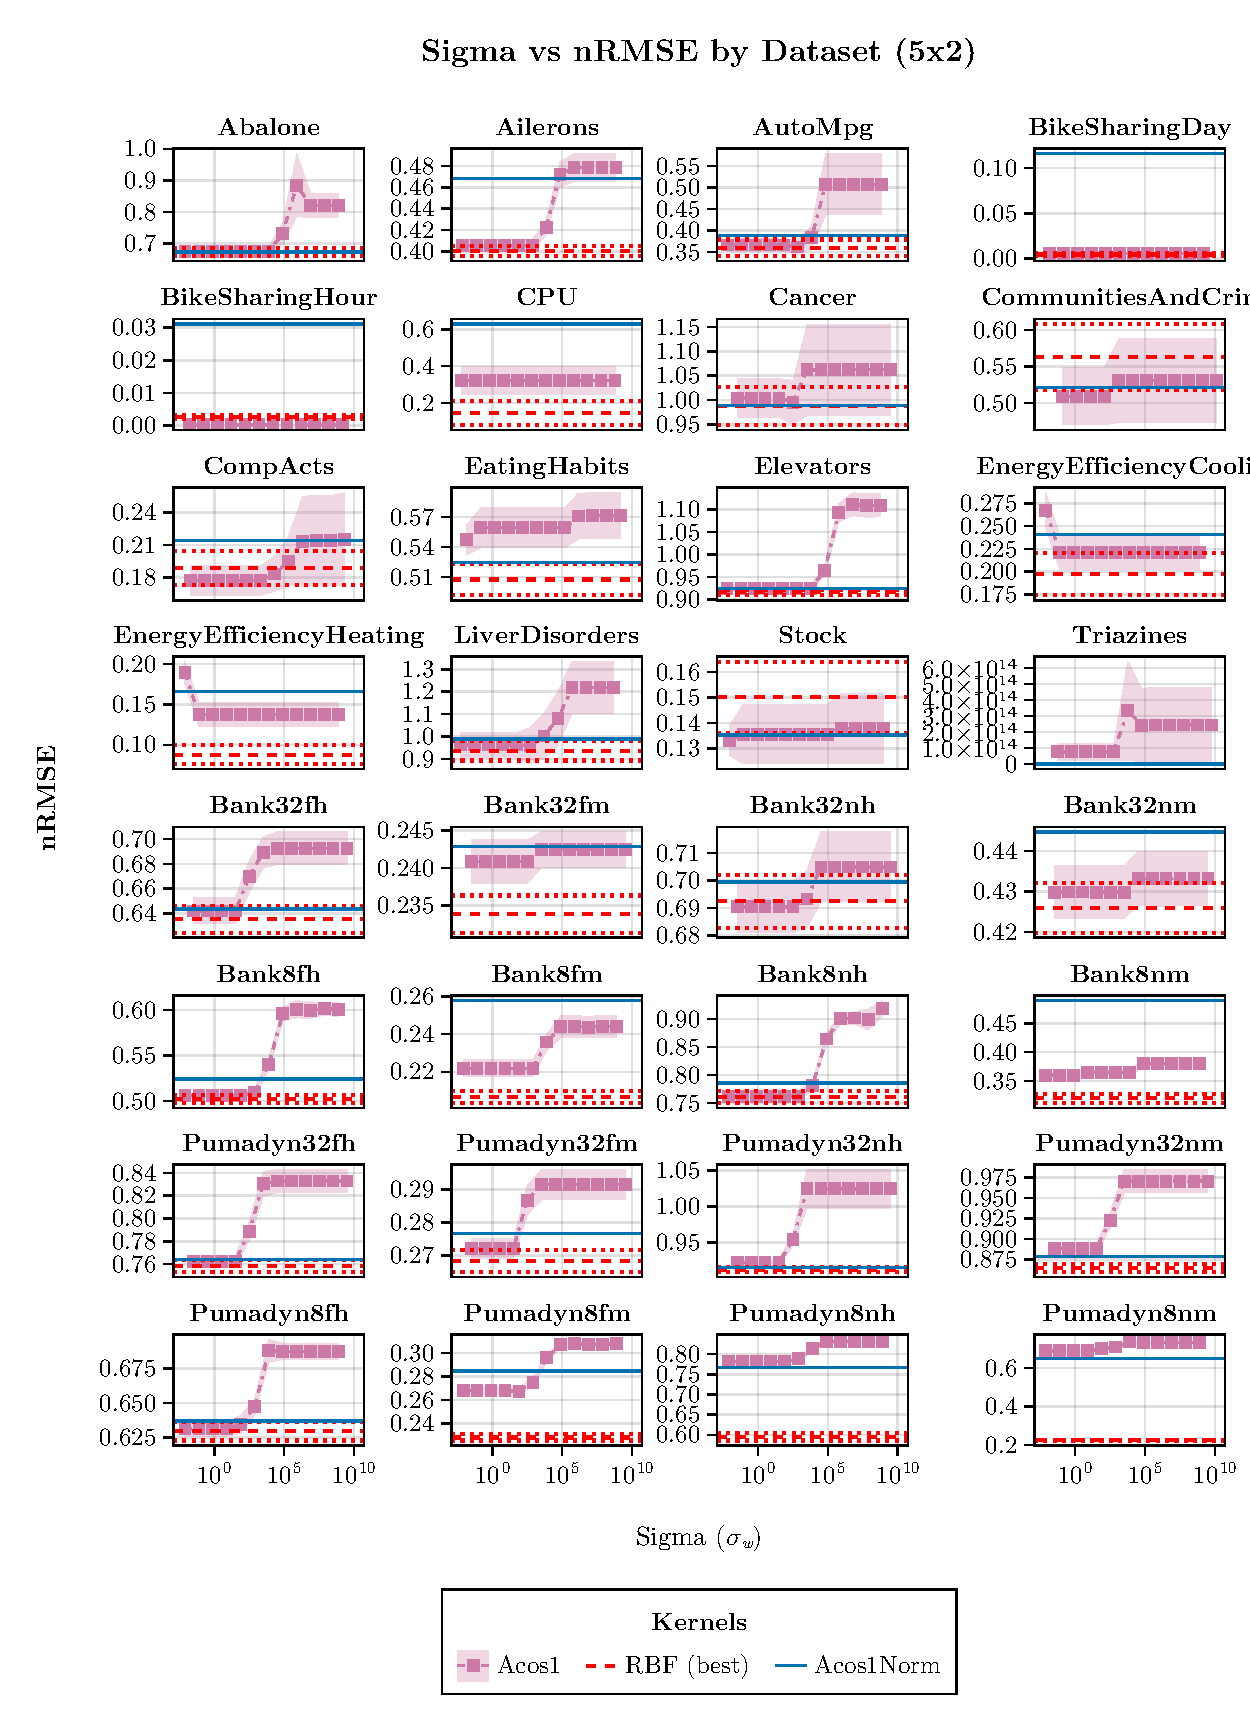
\includegraphics[width=\textwidth]{plots/nRMSE_acos1_scaled}
    \caption{Sigma vs Normalized Root Mean Squared error by dataset using non-normalized arccosine kernel for $n=1$}%
    \label{fig:nrmse-acos1-scaled}
\end{figure}

It seems that lover values of $\sigma$ are better for the non-normalized arccosine
kernel for $n=1$. Additionally, the normalized arccosine kernel for $n=1$ seems
to not perform as well as the non-normalized version with proper tuning of the
$\sigma$ hyperparameter. There are some datasets in which the performance of
both the normalized and non-normalized arccosine kernel for $n=1$ is significantly
worse than the RBF kernel. This is the case for \texttt{Bank8nm}, \texttt{Bank8fm},
\texttt{Pumadyn8fm}, \texttt{Pumadyn8nh}, \texttt{Pumadyn8nm} and \texttt{EnergyEfficiencyHeating}.

There is an issue with \texttt{Triazines}, where the value of the nRMSE is well
above 1 ($10^{14}$). This may be caused by the fact that the dataset is very small
(186 instances) but has a relatively large number of features (60) and may cause numerical
issues when computing the angles between the vectors.

\subsubsection{Arccosine kernel for $n=2$}

For the arccosine kernel with $n=2$, not all datasets could be computed due to
time constraints. As explained above, for some datasets, the SMO algorithm
took too long to converge. \Cref{fig:nrmse-acos2-scaled} shows the results for
the non-normalized arccosine kernel for $n=2$ for the different datasets which
could be computed. Again the performance of the normalized arccosine kernel for
$n=2$ and the RBF kernel are also shown.

\begin{figure}[H]
    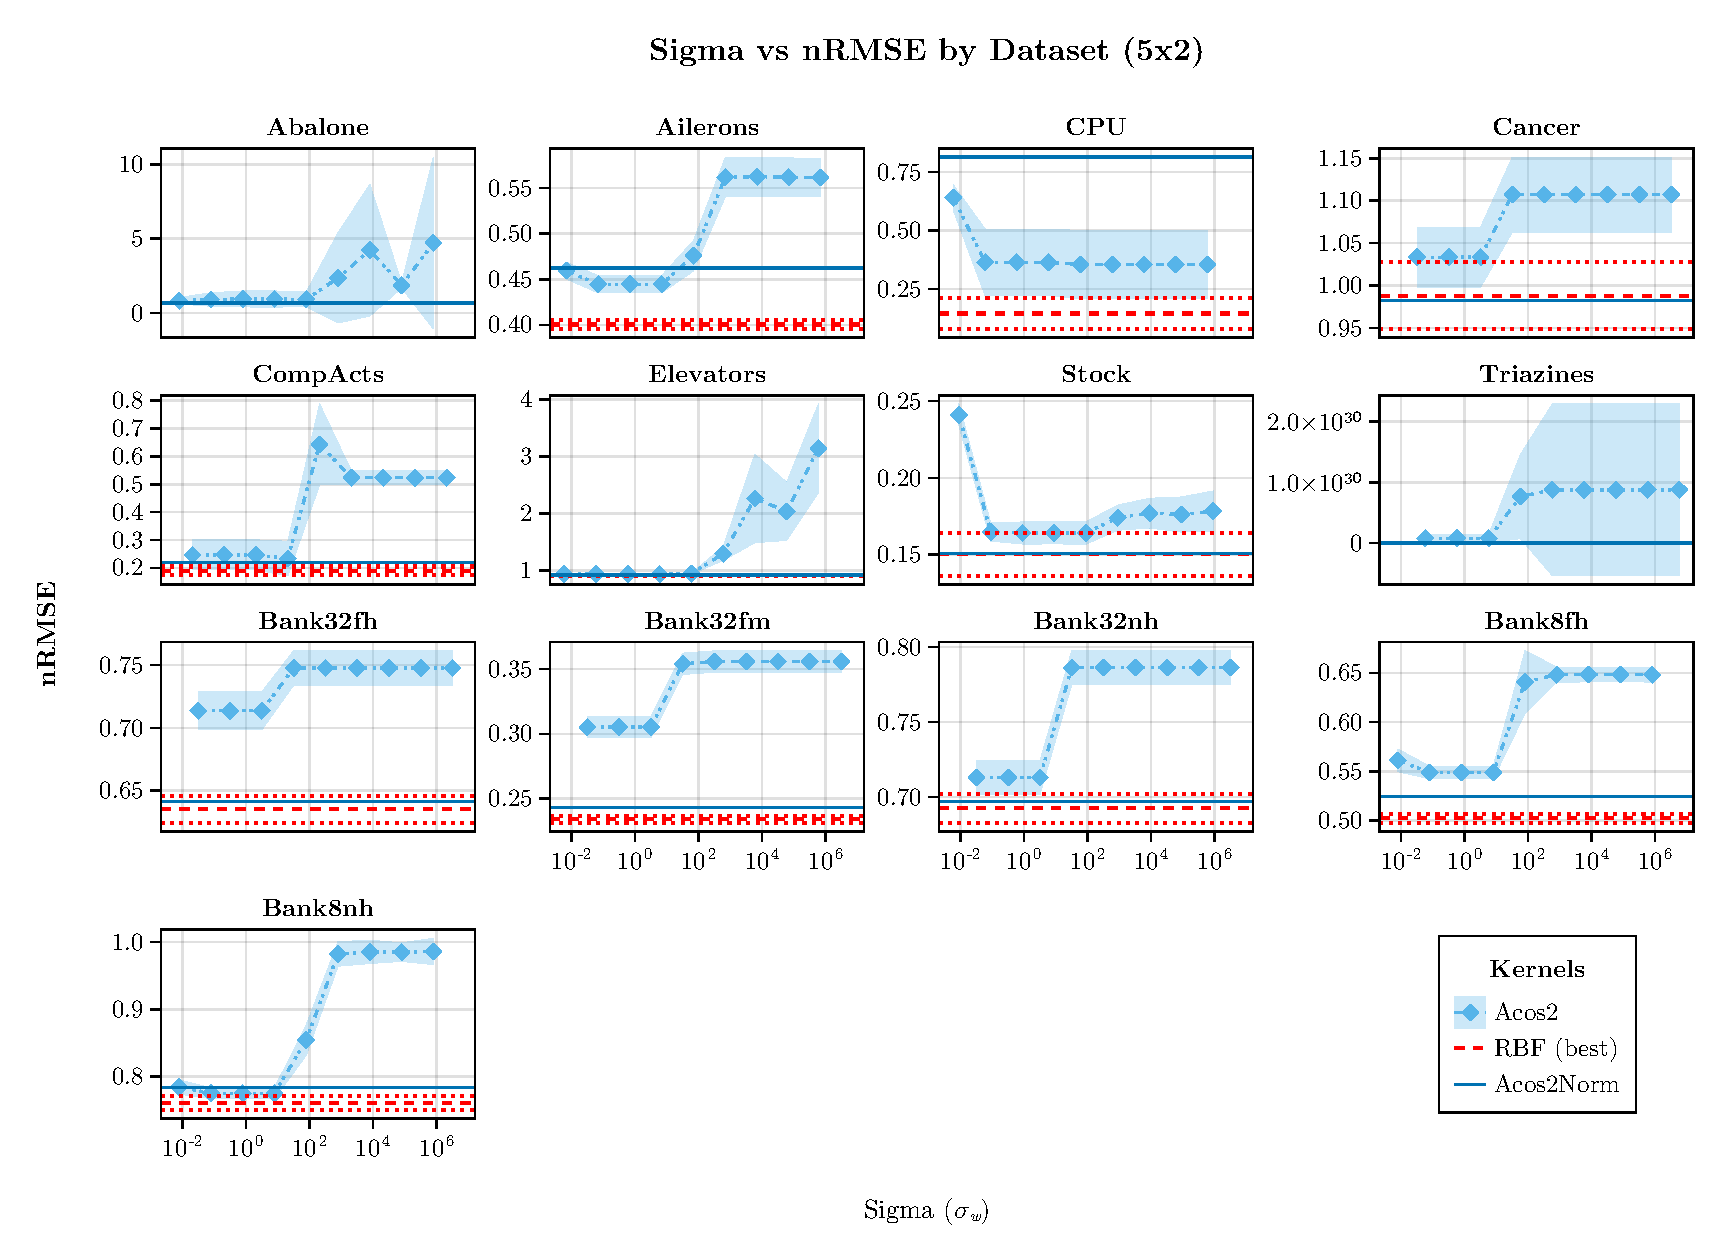
\includegraphics[width=\textwidth]{plots/nRMSE_acos2_scaled}
    \caption{Sigma vs Normalized Root Mean Squared error by dataset using non-normalized arccosine kernel for $n=2$}%
    \label{fig:nrmse-acos2-scaled}
\end{figure}

With this kernel, there are various datasets which present issues (values of nRMSE
above 1). This is the case for \texttt{Abalone}, \texttt{Cancer}, and \texttt{Triazines}.

There are clearly some issues with the non-normalized arccosine kernel for $n=1$ and
specially for $n=2$. We suspect that without normalization, the differences between
the values of the features are too large in some datasets, leading to numerical errors.

If we try to visualize the kernel for $n=1$ and $n=2$ in a 3-dimensional space around
the origin, we can observe how for relatively small differences between $x$ and $y$,
the value of the kernel is very large. This is shown in \cref{fig:kernel-acos1-3d,fig:kernel-acos2-3d}.
This specially noticeable for $n=2$ where it grows exponentially. This is due to the
nature of the kernels which come from the \emph{Ramp} (or \emph{ReLU}) and
\emph{Quarter-Pipe} (or \emph{RePU}) activation functions which we discussed in
\cref{sec:arc_cosine_kernels}.

\begin{figure}[H]
    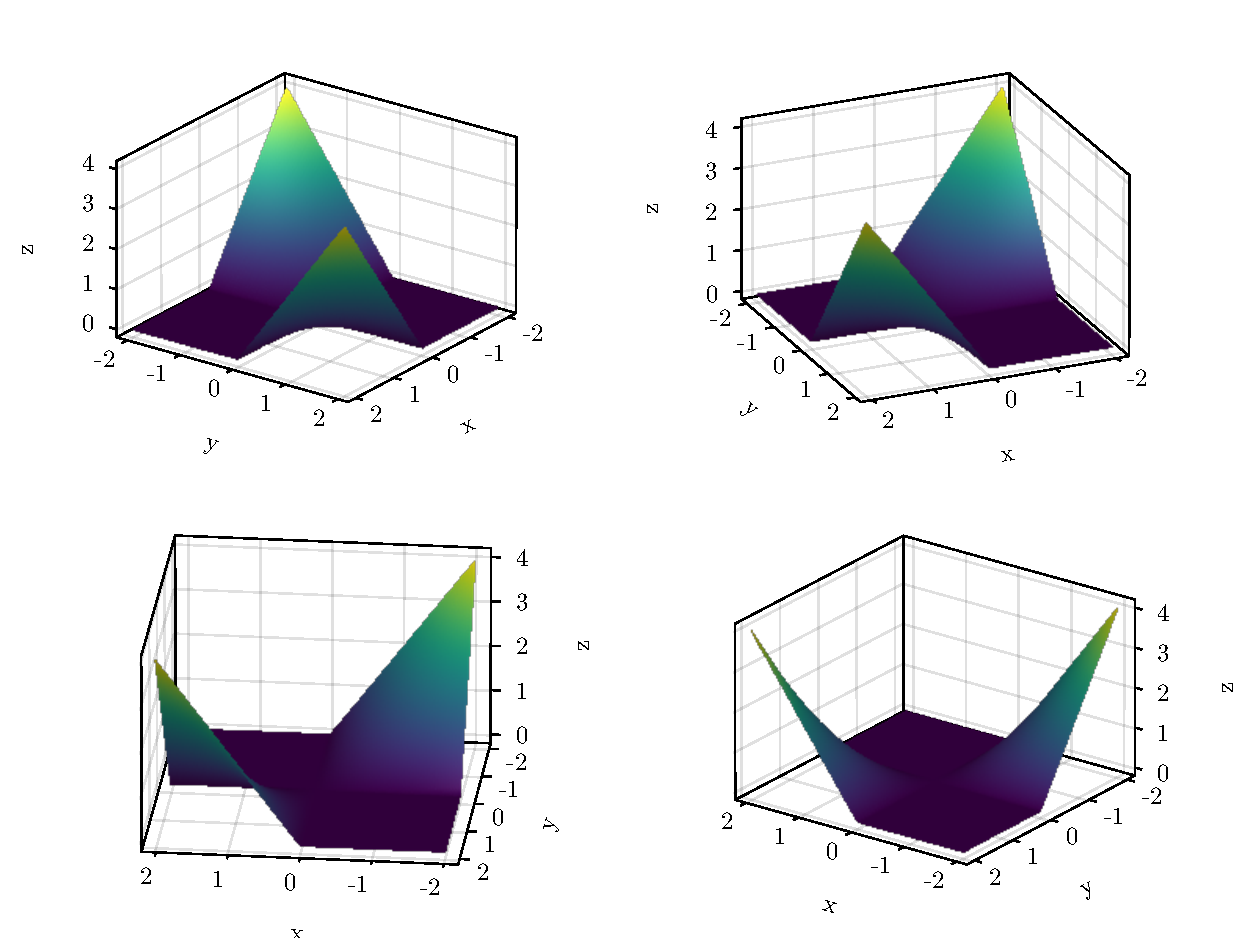
\includegraphics{plots/kernel_acos1_3d}
    \caption{3D visualization of acos kernel $n=1$ around the origin}
    \label{fig:kernel-acos1-3d}
\end{figure}

\begin{figure}[H]
    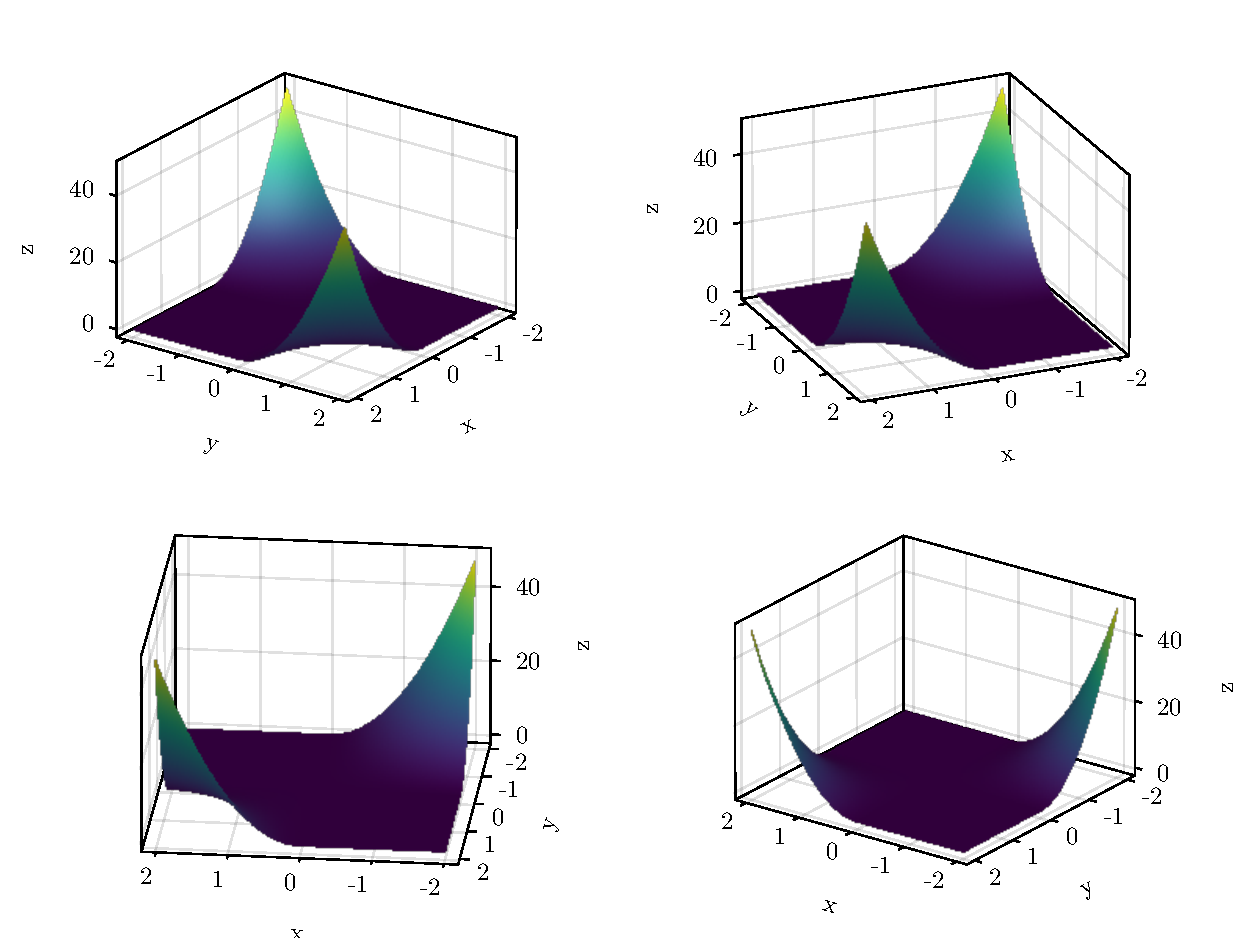
\includegraphics{plots/kernel_acos2_3d}
    \caption{3D visualization of acos kernel $n=2$ around the origin}
    \label{fig:kernel-acos2-3d}
\end{figure}
